\documentclass[a4paper]{report}
\usepackage[utf8]{inputenc}
\usepackage[spanish]{babel}
\usepackage[dvipsnames]{xcolor}
\usepackage{parskip}
\usepackage[colorlinks=true,urlcolor=blue,linkcolor=black]{hyperref}
\usepackage{url}
\usepackage{float}
\usepackage{amsmath,amssymb}
\usepackage{graphicx}
\usepackage{geometry}
\usepackage{caption}
\usepackage{wrapfig}
\usepackage{fancyvrb}
\usepackage{lmodern}
\usepackage{color,array}
\usepackage{etoolbox}
\usepackage{minted}
\usepackage{xpatch}
\usepackage{subfig}
\usepackage{colortbl}
\usepackage{tikz}
\usetikzlibrary{calc,tikzmark,arrows}
\usepackage{svg}
\usepackage{color,soul}
\usepackage{tcolorbox}

% mips-lexer.py HAS TO HAVE execution permissions for this to work
% minted uses which to detect the file:
% https://github.com/gpoore/minted/blob/d46f1ba2d248f2f3504bcc795dd39c613bd3c5a0/source/minted.sty#L197
\renewcommand{\MintedPygmentize}{./mips-lexer.py}

\makeatletter
\patchcmd{\@makechapterhead}{\vspace*{50\p@}}{}{}{}% Removes space above \chapter head
\patchcmd{\@makeschapterhead}{\vspace*{50\p@}}{}{}{}% Removes space above \chapter* head
\makeatother

\xpretocmd{\chapter}{\setcounter{section}{0}}{}{}

\unaccentedoperators

\definecolor{autumn-red-pyg}{HTML}{AA0000}
\definecolor{autumn-blue-pyg}{HTML}{0000AA}
\definecolor{autumn-gray-pyg}{HTML}{AAAAAA}
\definecolor{autumn-teal-pyg}{HTML}{00AAAA}
\definecolor{murphy-green-pyg}{HTML}{008000}
\definecolor{murphy-periwinkle-pyg}{HTML}{ABABFF}
\definecolor{murphy-deepsea-pyg}{HTML}{005487}

\setlength{\textfloatsep}{0pt}
\counterwithout{section}{chapter}
\usemintedstyle{default}

\title{\Huge{}\texttt{MIPS R2000}\\\vspace{8pt}\Large{}\textbf{\scalebox{.85}[1.0]{Práctica 1}}}
\author{Ariel Leonardo Fideleff}

\begin{document}

\pagenumbering{gobble}
\maketitle

\chapter{Cuestiones}

\section{Apartado 1}

\begin{center}
\large\textbf{-- \textsl{Declaración de palabras en memoria} --}
\end{center}

\subsection*{1.1 y 1.2}

Como podemos ver en la Figura \ref{fig:c1-1}, los dos números enteros reservados en el programa se ubicaron en las posiciones \texttt{0x10010000} y \texttt{0x10010004}, distanciados justamente por 4 bytes ya que se corresponde con el tamaño de palabra. Es decir, si cada entero fue reservado como un \mintinline{mips}{.word}, cada uno ocupa 4 bytes. Con esto, sumado a que el ensamblador los coloca uno seguido del otro en la memoria, dado que el primer valor por defecto comienza en la posición \texttt{0x10010000}, el segundo necesariamente deberá ubicarse 4 posiciones de memoria después (cada posición se corresponde con un byte).

En cuanto a los valores como tal, podemos ver la diferencia en que hayamos indicado uno en decimal, mientras el otro en hexadecimal. De esta forma, el número 15 en decimal es representado como \texttt{0x0000000f} en hexa, forma con la cual se presenta en el panel de datos. Mientras, el segundo valor, al haber sido especificado en el programa en base 16, lo reconocemos fácilmente como \texttt{0x00000015} en el panel en cuestión.

\begin{figure}[h]
    \centering
    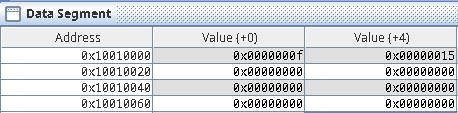
\includegraphics[width=.7\linewidth]{img/c1-1}
    \caption{Datos del programa según se indican en el panel de datos}
    \label{fig:c1-1}
\end{figure}

\subsection*{1.3}

De acuerdo a lo dicho en la teoría, las etiquetas \texttt{palabra1} y \texttt{palabra2} deberían tomar el valor de las posiciones de memoria a las que hacen referencia. En este caso, las ya mencionadas \texttt{0x10010000} y \texttt{0x10010004}, respectivamente.

De hecho, como se muestra en la Fig. \ref{fig:labels-fst}, esto lo podemos comprobar en la ventana \textit{Labels}, que se puede activar desde la configuración del simulador.

\begin{figure}[h]
    \centering
    \captionsetup{justification = centering}
    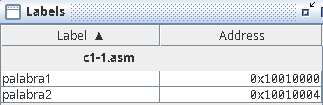
\includegraphics[width=.5\linewidth]{img/c1-3}
    \caption{Valores de las etiquetas \texttt{palabra1} y \texttt{palabra2} en la ventana \textit{Labels}}
    \label{fig:labels-fst}
\end{figure}

\subsection*{1.4}

Al ensamblar el programa dado, no parece presentar ninguna diferencia con respecto al primer programa visto, ya sea tanto en la memoria, como también en otras variables visibles en el simulador (por ejemplo, los registros).

\subsection*{1.5}

El siguiente código cumple con la consigna planteada:

\vspace{7pt}
\inputminted[linenos]{mips}{src/cuestiones/c1-5.asm}
\vspace{7pt}

Y en la Figura \ref{fig:arr5-mem} podemos comprobar que los valores fueron almacenados de forma correcta, considerando que los números 30 y 60 en decimal se corresponden con \texttt{0x0000001e} y \texttt{0x0000003c} en hexadecimal, respectivamente.

\begin{figure}[h]
    \centering
    \captionsetup{justification = centering}
    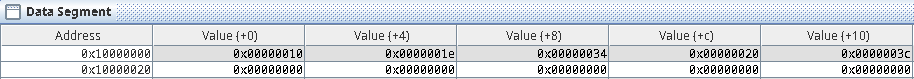
\includegraphics[width=.95\linewidth]{img/c1-5a}
    \caption{Valores del vector de números declarado en el programa propuesto, según se indican en el panel de datos}
    \label{fig:arr5-mem}
\end{figure}

Notar que al haber cambiado la dirección de memoria inicial donde se quiere que se almacenen los datos (respecto a la utilizada por defecto), debimos de expandir el panel de datos del simulador para poder visualizar el segmento de la memoria donde se ubicaban los valores reservados de nuestro vector, seleccionando la opción correspondiente desde un menú desplegable, tal como se lo muestra en la Figura \ref{fig:dropdown-data}.


\begin{figure}[h]
    \centering
    \captionsetup{justification = centering}
    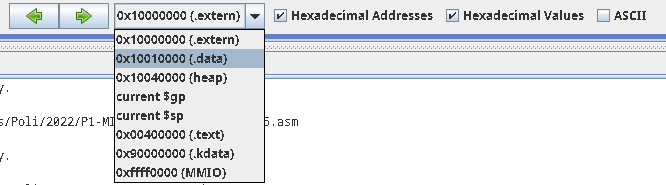
\includegraphics[width=.7\linewidth]{img/c1-5b}
    \caption{Menú desplegable para seleccionar la visualización del segmento de memoria correspondiente al utilizado por el programa planteado}
    \label{fig:dropdown-data}
\end{figure}

\subsection*{1.6}
\label{sec:c1-6}

Podemos probar cambiar el argumento de la directiva \mintinline{mips}{.data} para intentar almacenar los datos partiendo desde la dirección \texttt{0x10000002}:

\vspace{7pt}
\inputminted[linenos]{mips}{src/cuestiones/c1-6.asm}
\vspace{7pt}

Hecho este cambio, el panel de datos nos muestra que los valores ahora son almacenados partiendo desde la dirección de memoria \texttt{0x10000004}, saltando de 4 en 4 (por el tamaño de palabra, Fig. \ref{fig:not-multiple}).

\begin{figure}[h]
    \centering
    \captionsetup{justification = centering}
    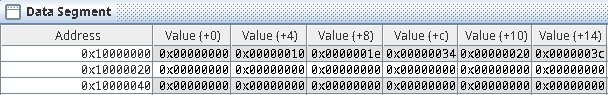
\includegraphics[width=.8\linewidth]{img/c1-6}
    \caption{Valores y respectivas posiciones de memoria del programa con argumento de \mintinline{mips}{.data} modificado}
    \label{fig:not-multiple}
\end{figure}

Esto difiere en principio de lo que uno podría esperar, ya que se le está indicando al ensamblador que ubique la información partiendo desde la dirección de memoria \texttt{0x10000002}. El motivo por el cual ejecuta el cambio descripto, es porque se requiere que la ubicación de todos los valores se encuentren en posiciones múltiplos de 4, de forma que la memoria ``esté alineada''. Éste es un requisito de la arquitectura MIPS, o bueno, al menos estamos seguros basándonos en lo visto en la teoría, que lo es para el lenguaje de máquina de los microprocesadores MIPS R2000.

Con esto en cuenta, el ensamblador, sabiendo que indicamos el espacio para datos partiendo desde la posición de memoria \texttt{0x10000002}, buscó por la posición de memoria (mayor o igual) múltiplo de 4 más cercana, y a partir de allí ubicó los valores del vector de números reservado en el programa.

\begin{center}
\large\textbf{-- \textsl{Declaración de bytes en memoria} --}
\end{center}

\subsection*{1.7 y 1.8}

\begin{wrapfigure}[11]{r}{.25\linewidth}
    \centering
    \captionsetup{justification = centering}
    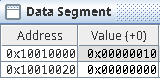
\includegraphics[width=\linewidth]{img/c1-7}
    \caption{Representación del contenido especificado en la memoria, visto desde el panel de datos}
    \label{fig:c1-7}
\end{wrapfigure}

Como ya sabemos, al no especificar ningún argumento para la directiva \mintinline{mips}{.data}, los datos se ubicarán partiendo desde la dirección de memoria \texttt{0x10010000} por defecto.

Además, al tratarse de un único byte, y considerando que el valor indicado \texttt{0x10} no supera el tamaño permitido por la directiva (el máximo valor posible sería \texttt{0xFF}), éste se almacenaría ``al comienzo de la palabra'', efectivamente implicando que el valor de la palabra que contiene el byte sea el mismo al especificado. Al fin y al cabo, el tamaño de una palabra es mayor al de un byte (justamente, 4 bytes), por lo que resulta en que el valor de la palabra sea el mismo al valor del tamaño de un byte, antecedido por 0s que no cambian el entero final almacenado.

\subsection*{1.9 y 1.10}
\label{sec:c1-10}

En este caso, se almacenan los valores \textbf{\texttt{0x40302010}} y \textbf{\texttt{0x10203040}} en las posiciones de memoria \textbf{\texttt{0x10010000}} y \textbf{\texttt{0x10010004}} respectivamente.

Si bien el segundo valor es indicado como tal de forma explícita en el código presentado, el primer valor, en cambio, es el resultado de almacenar un vector de 4 valores especificados del tamaño de 1 byte. Esto nos muestra que el simulador, por un lado, almacena los valores indicados con la directiva \mintinline{mips}{.byte} de forma contigua, independientemente de que los valores sean accedidos de a una palabra a la vez. Por otro lado, nos indica también el orden que utiliza para guardar los datos dentro de una palabra, el cual puede ser identificado afín con el concepto de \textit{Little-Endian}, el cual consiste en la organización y alineamiento de los datos de forma que, aplicado a este caso, ``lo que va primero'' se almacene en las direcciones de memoria más bajas, y así en adelante.\footnote{Más formalmente, el concepto de \textit{Little Endian} hace referencia a que los bytes menos significativos dentro de una palabra sean almacenados en posiciones de memoria más chicas, relacionándose principalmente con la forma en la que se \textit{internamente} se manejan y ordenan los bytes de una palabra.}

Esta conclusión la podemos obtener partiendo, primero, en que sabemos que el valor presentado en el panel de datos de una palabra \texttt{0xXXXXXXXX}, se corresponde con la representación en hexadecimal de los bytes en posiciones de memoria menores a mayores, interpretadas de derecha a izquierda. Para probar esto, podemos modificar el programa descripto para la consigna, y especificar que los datos se ubiquen partiendo desde la dirección de memoria \texttt{0x10010002}:

\vspace{7pt}
\inputminted[linenos]{mips}{src/cuestiones/c1-10.asm}
\vspace{7pt}

Con este cambio, la palabra en la dirección \texttt{0x10010000} almacena ahora el valor \texttt{0x20100000}, a la vez que la palabra en la dirección \texttt{0x10010004} almacena los dos valores restantes del vector de \mintinline{mips}{.byte} (valor \texttt{0x00004030}, ver Fig. \ref{fig:bytes-shift-endian}), demostrando cómo los bytes se corrieron dos posiciones desde la derecha (posiciones como bytes, que en hexadecimal se corresponde con dos dígitos, así representando un espacio de 4 dígitos para haber cambiado la dirección de memoria de \mintinline{mips}{.data} dos posiciones adelante de la usada por defecto).

\begin{figure}[h]
    \centering
    \captionsetup{justification = centering}
    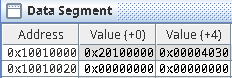
\includegraphics[width=.4\linewidth]{img/c1-10}
    \caption{Valores de las palabras en memoria correspondientes al vector de \mintinline{mips}{.byte}, tras indicar que los datos se almacenen desde la posición \texttt{0x10010002}}
    \label{fig:bytes-shift-endian}
\end{figure}

Teniendo esto en cuenta, vemos que los valores del vector de \mintinline{mips}{.byte} fueron almacenados en orden creciente respecto a posiciones de memoria que también crecen. Así, como en el programa indicamos los números \texttt{0x10}, \texttt{0x20}, \texttt{0x30} y \texttt{0x40} (en este orden), el primero de todos, el \texttt{0x10}, se encuentra en la posición de memoria \texttt{0x10010000}, luego el \texttt{0x20} en la posición \texttt{0x10010001}, y así sucesivamente.

Por ende, leemos el vector completo como el valor de una palabra \texttt{0x40302010} (siendo 4 elementos, exactamente la misma cantidad como hay de bytes en una palabra, siendo una sola suficiente para representar la totalidad de dicho vector). Mientras, guardar el valor \texttt{0x10203040} nos da una la pauta de cómo se hubieran almacenado los valores del vector en cuestión si el ensamblador hubiera tenido un comportamiento que se acercara a \textit{Big-Endian} (en el cual los ``últimos números'' se guardarían en las posiciones de memoria más pequeñas/bajas).

\subsection*{1.11}

A pesar del comportamiento de juntar los valores del tamaño de 1 byte en palabras, esto no afecta sobre los valores de las etiquetas \texttt{palabra1} y \texttt{palabra2}, que indican la primera posición de memoria desde la cual parte cada valor (en este caso, digamos, el vector y el segundo valor). Además, ayuda que puntualmente el vector definido en la consigna pueda estar contenido en una sola palabra, como ya mencionamos.

Por lo tanto, las etiquetas \texttt{palabra1} y \texttt{palabra2} toman los valores \texttt{0x10010000} y \texttt{0x10010004} respectivamente.

\begin{center}
\large\textbf{-- \textsl{Declaración de cadenas de caracteres} --}
\end{center}

\subsection*{1.12}

Para localizar la cadena ingresada en el programa dentro de la memoria, sabemos que debería de comenzar en la posición \texttt{0x10010000} ya que, como venimos repitiendo, es la dirección por defecto donde comienzan los datos si no se le provee un argumento a la directiva \mintinline{mips}{.data}.

Observando la valor de la palabra en la dirección mencionada, nos encontramos con el valor \textbf{\texttt{0x64636261}}. El patrón que tiene este valor es familiar con el explorado en la sección interior, en el cual veíamos cómo múltiples bytes estaban almacenados dentro de una palabra. Con esto en cuenta, podemos pensar que ésta posiblemente contenga los bytes individuales \texttt{0x61}, \texttt{0x62}, \texttt{0x63} y \texttt{0x64}, leyendo de posiciones menores a mayores en memoria. Considerando que la forma en que estos valores crecen se asemeja mucho con cómo nuestra cadena contiene caracteres consecutivos y lexicográficamente crecientes, sumado a que el nombre de la directiva utilizada en el programa para almacenar la cadena recibe el nombre de \mintinline{mips}{.ascii}, es intuitivo pensar que los bytes antes identificados se correspondan con las letras de la cadena en cuestión.

Comprobando nuestras sospechas, \texttt{0x61} equivale al número \texttt{97} en decimal, número correspondiente a la letra \texttt{\textquotesingle{}a\textquotesingle{}} en el código ASCII. Sucesivamente el resto de bytes equivalen en decimal entonces a los números \texttt{98}, \texttt{99} y \texttt{100}, correspondientes a las letras \texttt{\textquotesingle{}b\textquotesingle{}}, \texttt{\textquotesingle{}c\textquotesingle{}} y \texttt{\textquotesingle{}d\textquotesingle{}} en ASCII.

\begin{figure}[h]
    \centering
    \captionsetup{justification = centering}
    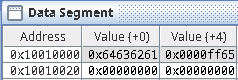
\includegraphics[width=.4\linewidth]{img/c1-12}
    \caption{Valores en memoria tras el ensamblado del código indicado}
    \label{fig:ascii-mem}
\end{figure}

De todas formas, debemos recordar que nuestra cadena era \texttt{\char34{}abcde\char34}, por lo que nos estaría faltando ubicar la letra \texttt{\textquotesingle{}e\textquotesingle{}}. Como podemos ver en la Figura \ref{fig:ascii-mem}, la próxima palabra en la posición \texttt{0x10010004} contiene el valor \textbf{\texttt{0x0000ff65}}. El \textsl{\texttt{65}} en las posiciones menos significativas del valor surge como continuación de la cadena de caracteres, el cual se encuentra en la posición de memoria siguiente al \textsl{\texttt{64}} de la palabra anterior, pero que se nos muestra de esta forma al tener que ubicarse por fuera del espacio de la primera palabra (en simples palabras, ``no entraba'' en la primera palabra), y por lo ya discutido en la sección anterior.

Luego, el \textsl{\texttt{ff}} que le sigue al \textsl{\texttt{65}} se corresponde con el valor almacenado con la directiva \mintinline{mips}{.byte} dentro del programa.

\subsection*{1.13}

Si empleamos la directiva \mintinline{mips}{.asciiz} en vez de la directiva \mintinline{mips}{.ascii} en el programa de la Cuestión anterior, el cambio que se observa es el agregado de lo que sería el equivalente a un byte \textit{vacío} entre el final de la cadena, y el próximo valor almacenado con la directiva \mintinline{mips}{.byte}. Es decir, mientras la primera palabra no cambia, la segunda en memoria toma ahora el valor \textbf{\texttt{0x00ff0065}}.

Este compartamiento es similar a la forma en la que, en lenguajes de programación como \texttt{C}, se agrega un caracter con valor ASCII = 0 al final de una cadena, conocido como el \textit{terminador} (generalmente representado como {\usemintedstyle{default}\mintinline{mips}{'\0'}}). Haciendo uso de este caracter, se puede determinar en qué punto finaliza una cadena de caracteres, incluso conociendo sólo el comienzo de la misma y que sus elementos se encuentran en posiciones de memroia consecutivas. Por lo tanto, al operar con ella, es sólo cuestión de recorrer todas estas posiciones partiendo desde la primera, hasta encontrarse con un byte \texttt{0x00} que indica el final.

\subsection*{1.14}

Podemos reemplazar la directiva \mintinline{mips}{.ascii} con la \mintinline{mips}{.byte} cargando posiciones en memoria con un vector de los caracteres de la cadena original, representados con su valor ASCII:

\vspace{7pt}
\inputminted[linenos]{mips}{src/cuestiones/c1-14.asm}
\vspace{7pt}

De hecho, podemos incluso utilizar los caracteres como tales, en vez de sus equivalentes en ASCII, y el ensamblador se encargará de transformarlos en sus valores numéricos correspondientes:

\vspace{7pt}
\inputminted[linenos]{mips}{src/cuestiones/c1-14b.asm}
\vspace{7pt}

\begin{center}
\large\textbf{-- \textsl{Reserva de espacio en memoria} --}
\end{center}

\subsection*{1.15 y 1.16}

Observando el panel de datos con los valores en la memoria (Fig. \ref{fig:space-mem}), podemos ver que se ha reservado el tamaño equivalente a exactamente dos palabras, para la variable \texttt{espacio}. Esto equivale a 8 bytes, entendiéndose así que el parámetro de la directiva \mintinline{mips}{.space} está expresado en cantidad de bytes que se quiere reservar en memoria.

Dicho esto, entonces el rango de posiciones que se han reservado en la memoria para la variable es [\texttt{\textbf{0x10010004}}, \texttt{\textbf{0x1001000b}}]. Las palabras en posiciones \texttt{0x10010000} y \texttt{0x1001000c} contienen los valores \texttt{0x20} y \texttt{0x30} respectivamente, declarados con la directiva \mintinline{mips}{.word} en el programa.

\begin{figure}[H]
    \centering
    \captionsetup{justification = centering}
    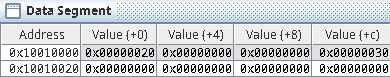
\includegraphics[width=.6\linewidth]{img/c1-15}
    \caption{Valores en memoria tras ensamblar el programa dado}
    \label{fig:space-mem}
\end{figure}

\begin{center}
\large\textbf{-- \textsl{Alineación de datos en memoria} --}
\end{center}

\subsection*{1.17}

Se reservó el rango de posiciones [\texttt{\textbf{0x10010001}}, \texttt{\textbf{0x10010004}}] en memoria para la variable \texttt{espacio}.

\subsection*{1.18}
\label{sec:c1-18}

Si bien los cuatro bytes reservados podrían contener la información de una palabra, éstos no podrían funcionar como tal ya que, como dijimos en la \hyperref[sec:c1-6]{Cuestión 1.6}, la memoria de una palabra tiene que \textit{estar alineada}, en el sentido que cada una debe comenzar en una posición de memoria múltiplo de 4.

Desde lo visto en la teoría, la arquitectura de MIPS nos permite leer información de la memoria de a una palabra a la vez, pues su tamaño equivale al ancho del bus de datos, y esto necesariamente debe ser en posiciones iniciales múltiplos de 4. Por tal motivo, si quisiérmos usar los 4 bytes reservados para \texttt{espacio} como un único espacio de memoria del tamaño de una palabra, realmente deberíamos acceder para cada operación necesaria a las palabras en las direcciones \texttt{0x10010000} y \texttt{0x10010004}, que lo hace poco práctico e ineficiente para este propósito. Esto sin mencionar las operaciones adicionales que se requerirían para juntar ambas palabras, o también descartar información en otras posiciones que se encuentren en las palabras, pero que no corresponda al espacio asignado para la tarea.

\subsection*{1.19}

El \texttt{byte1}, al haberse declarado al comienzo del programa, fue inicializado en la posición de memoria \textbf{\texttt{0x10010000}}. Mientras, como el \texttt{byte2} fue declarado al final del programa, éste fue posicionado en la dirección de memoria \textbf{\texttt{0x10010005}}, después del espacio reservado para la variable \texttt{espacio}.

\subsection*{1.20}

Finalmente, la variable \texttt{palabra} fue inicializada partiendo de la posición \texttt{\textbf{0x10010008}} en la memoria. Esto se debe a que como la variable fue declarada con la directiva \mintinline{mips}{.word}, ésta debe de ocupar una palabra entera, a pesar de que la memoria esté ocupada hasta la posición \texttt{0x10010005}. En consecuencia, la variable se ubica en la posición ya mencionada, teniendo en cuenta que la anterior palabra en la posición \texttt{0x10010004} tiene un byte ocupado por la variable \texttt{byte2}.

Esta situación es similar a la vista en la \hyperref[sec:c1-6]{Cuestión 1.6}, en el cual la declaración de una variable con \mintinline{mips}{.word} fue dada a partir del comienzo de la \textit{palabra} más próxima libre, en vez de comenzar desde la primera \textit{posición} libre.

\begin{figure}[H]
    \centering
    \captionsetup{justification = centering}
    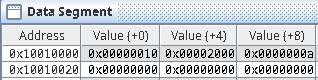
\includegraphics[width=.5\linewidth]{img/c1-17}
    \caption{Vista de la memoria posterior al emsamblado del código de las Cuestiones 1.17-1.20}
\end{figure}

\subsection*{1.21 y 1.22}

De haber entendido correctamente el rol de la directiva \mintinline{mips}{.align}, ésta hará que la próxima directiva de declaración de algún dato se coloque partiendo desde la próxima potencia de $2^n$, siendo n el argumento que recibe la directiva. En este caso, como la directiva recibe al número \textit{2} como argumento, la variable \texttt{espacio} se reservará partiendo desde la primera posición múltiplo de $2^2 = 4$ libre más cercana. Considerando que la primera posición de memoria libre a este punto es la \texttt{0x10010001} (ya que \texttt{byte1} ocupa la anterior), la próxima posición múltiplo de 4 disponible es la \texttt{0x10010004}. Podemos confirmar nuestra sospecha al ver el valor de la posición de memoria a la que hace referencia \texttt{espacio} en la ventana Labels (Fig. \ref{fig:c1-21-labels}).

\begin{figure}[h]
    \centering
    \captionsetup{justification = centering}
    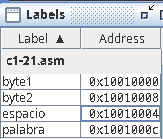
\includegraphics[width=.25\linewidth]{img/c1-21}
    \caption{Valores en memoria de las etiquetas para el código de las Cuestiones 1.21-1.22}
    \label{fig:c1-21-labels}
\end{figure}

Luego, como la directiva \mintinline{mips}{.space} recibe un \textit{4} como argumento, se reservan 4 posiciones desde la inicial, efectivamente inicializándose en el rango [\texttt{\textbf{0x10010004}}, \texttt{\textbf{0x10010007}}].

El hecho de reservar 4 posiciones de memoria (4 bytes), como también haber alineado la variable con una posición múltiplo de 4, hacen que el espacio reservado pueda constituir una palabra. No sólo el tamaño es igual al de una palabra (como ya vimos en la pregunta de la \hyperref[sec:c1-18]{Cuestión 1.18}), sino que también está alineada apropiadamente con el comienzo de una palabra. Al fin y al cabo, justamente es la directiva \mintinline{mips}{.align} la cual se encargó de hacerlo, ya que al indicarle el \textit{2} como argumento, alineó el espacio con una posición múltiplo de $2^2 = 4$, como es apropiado para una palabra (según lo discutido en la Cuestión mencionada).

Con todo esto en cuenta, podemos decir resumidamente que:

\begin{center}
    \textit{La directiva \mintinline{mips}{.align} ubica en memoria el próximo dato declarado a partir de la primera posición libre que sea múltiplo de $2^n$, siendo \textbf{n} el argumento pasado a la directiva.}
\end{center}

\section{Apartado 2}

\begin{center}
\large\textbf{-- \textsl{Carga de datos inmediatos (constantes)} --}
\end{center}

\subsection*{2.1}
\label{sec:c2-1}

La dirección de memoria donde se encuentra la instrucción en cuestión es la \texttt{\textbf{0x00400000}}, y ocupa el tamaño de exactamente una palabra (4 bytes = 32 bits). El valor que la representa es \texttt{0x3c108690}. Como sabemos que es una traducción de código en Assembly que conocemos, podemos deducir las partes que lo componen. Sin embargo, si bien algunas de ellas pueden ser reconocidas desde su representación en hexadecimal, deberemos de remitirnos a su equivalente en binario para darle completo sentido a cómo es que realmente funciona.

\begin{figure}[H]
    \centering
    \captionsetup{justification = centering}
    \texttt{\textbf{0\tikzmark{hex-lui-pref}x \textcolor{Red}{3c\tikzmark{hex-lui-tobin}10} \textcolor{Emerald}{86\tikzmark{hex-lui-ivalue}90}}}
    \begin{tikzpicture}[overlay, remember picture]
        \draw ($ (pic cs:hex-lui-pref) + (0,-.1) $) -- ($ (pic cs:hex-lui-pref) + (0,-.4) $) -| ($ (pic cs:hex-lui-pref) + (-3,-.6) $) node (pref) [label={[yshift=5pt]-90:\small{}\sffamily{}prefijo hexadecimal}] {};
        \draw ($ (pic cs:hex-lui-ivalue) + (0,-.1) $) -- ($ (pic cs:hex-lui-ivalue) + (0,-.4) $) -| ($ (pic cs:hex-lui-ivalue) + (3,-.6) $) node (ivalue) [label={[yshift=5pt]-90:\small{}\textcolor{Emerald}{\sffamily{}dato inmediato}}] {};

        \draw[-stealth] ($ (pic cs:hex-lui-tobin) + (0,-.1) $) -- ($ (pic cs:hex-lui-tobin) + (0,-.5) $) node (hex-tobin) [label={[yshift=2pt]-90:\textbf{\texttt{\textcolor{NavyBlue}{001\tikzmark{hex-lui-opcode}111}00\;000\textcolor{Purple}{10\tikzmark{hex-lui-reg}000}}}}] {};
        \draw ($ (hex-tobin) + (-.95,-.5) $) -- ($ (hex-tobin) + (-.95,-.7) $) -| ($ (hex-tobin) + (-2,-.9) $) node [label={[yshift=5pt]-90:\small\sffamily{}\textcolor{NavyBlue}{código de instrucción}}] {};
        \draw ($ (hex-tobin) + (1.075,-.5) $) -- ($ (hex-tobin) + (1.075,-.7) $) -| ($ (hex-tobin) + (2,-.9) $) node [label={[yshift=5pt]-90:\small\sffamily{}\textcolor{Purple}{número de registro}}] {};
    \end{tikzpicture}
    \vspace{50pt}
    \caption{Formato del valor contenido en memoria para la instrucción ingresada}
    \label{fig:lui-mem-hex}
\end{figure}

En la Figura \ref{fig:lui-mem-hex} vemos las 4 partes del valor en memoria para la instrucción:

\begin{itemize}
    \item El \textbf{prefijo hexadecimal}, el cual ya bien sabemos nos indica que un valor dado está representado en una notación numérica con base 16.
    \item El \textbf{código de instrucción} (conocido como \textit{opcode}), es decir, un valor que nos indica qué tipo de instrucción se está indicando a ejecutarse. En el código tratado, se corresponde con informar que se quiere llevar a cabo la instrucción \mintinline{mips}{lui}.

        El motivo por el cual para poder separar este campo debemos convertir en binario los primeros dos bytes de la palabra, es que el código de instrucción ocupa los primeros \textit{6} bits de la palabra. Por lo tanto, al pasarse a base 16, no es claramente distinguible. Por la misma razón así sucede con los siguientes dos grupos de 5 bits (el primero de ellos ignorado para la instrucción \mintinline{mips}{lui}).
    \item El \textbf{número de registro}, que contiene el identificador del registro al cual el dato inmediato será cargado. Si bien en código Assembly éste es representado con un nombre \mintinline{mips}{$s0}, internamente los registros son enumerados del 0 al 31, haciendo que esta abstracción sea interpretada por el ensamblador al cargarse la instrucción en memoria. De hecho, en el programa dado se puede reemplazar \mintinline{mips}{$s0} por \mintinline{mips}{$16} sin repercusiones.
    \item El \textbf{dato inmediato}, el cual como ya vimos en la teoría, es un valor del tamaño de media palabra (2 bytes = 16 bits), el cual será cargado en los 16 bits más significativos del registro especificado. Debido a su tamaño en bits múltiplo de 4, sumado a que se lo representa en el código en hexadecimal dentro del código en cuestión, lo hace fácil de distinguir en la representación en hexa del valor en memoria.
\end{itemize}

\subsection*{2.2}

Efectivamente, al correr el programa, los primeros 2 bytes del registro son cargados con el valor \texttt{0x8690}, así quedando la palabra almacenada en el registro como \textbf{\texttt{0x86900000}}.

\subsection*{2.3 y 2.4}
\label{sec:c2-4}

De forma similar a la Cuestión anterior, el dato inmediato especificado como argumento a la instrucción \mintinline{mips}{li} es cargado en el registro indicado como argumento. La diferencia es que este valor es del tamaño de una palabra completa, en vez de media palabra como sucedía con la instrucción \mintinline{mips}{lui}.

Ante esto, tras revisar la interpretación del código ensamblado en el panel de texto (\textit{Text Segment}), vemos que, siendo que \mintinline{mips}{li} es realmente una \textit{pseudoinstrucción}, fue descompuesta en dos instrucciones del procesador: la ya vista \mintinline{mips}{lui}, y otra llamada \mintinline{mips}{ori}.\\

Conociendo ya el funcionamiento de \mintinline{mips}{lui} en base a lo visto en la Cuestión anterior, podemos entender que carga los primeros dos bytes (es decir, los más significativos) del valor inmediato utilizado en el código, al registro \mintinline{mips}{$at} (abreviación de \textit{Assembler Temporary}). Este registro está reservado por el ensamblador para las operaciones realizadas como \textit{pseudo comandos}, es decir, operaciones intermedias llevadas a cabo por las instrucciones reales que fueron obtenidas de la interpretación de una instrucción en el código Assembly.\footnote{\url{https://en.wikibooks.org/wiki/MIPS_Assembly/Register_File}} La interpretación de pseudoinstrucciones suele involucrar el uso del registro \mintinline{mips}{$at}, como es el caso en cuestión.


Posteriormente, se hace uso de la instrucción \mintinline{mips}{ori}, también llamada \textit{OR Immediate}, el cual dado un registro de destino, un registro origen y un valor inmediato, almacena el resultado de la operación \texttt{OR} binaria entre los últimos dos, en el registro de destino. El valor inmediato dicho debe de tener un tamaño de, al igual que en \mintinline{mips}{lui}, media palabra. Por lo tanto, en este caso, al correr esta instrucción se procede a almacenar en el registro de destino, originalmente especificado en la pseudoinstrucción \mintinline{mips}{li}, el resultado de hacer el \texttt{OR} binario entre:

\begin{itemize}
    \itemsep0em
    \item Los dos bytes menos significativos del valor que se quería cargar originalmente al registro en el programa.
    \item Los otros dos bytes anteriormente almacenados en \mintinline{mips}{$at} con la instrucción real \mintinline{mips}{lui}.
\end{itemize}

Notar que, como la instrucción \mintinline{mips}{lui} establece los otros dos bytes menos significativos de \mintinline{mips}{$at} en 0, aplicar a continuación la operación \texttt{OR} no afectará al valor inmediato con el que se opera, resultando en lo que podría considerarse como ``la carga de un valor'' para estos dos bytes.

\begin{figure}[h]
    \centering
    \captionsetup{justification = centering}
    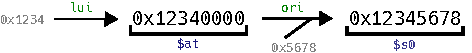
\includegraphics[width=.6\linewidth]{img/c2-4.pdf}
    \caption{\mintinline{mips}{li $s0, 0x12345678}, con las instrucciones reales que lo implementan}
\end{figure}

Pensando más a fondo, resulta claro el motivo de tener una pseudoinstrucción tal como \mintinline{mips}{li}. Y es que, con un tamaño de palabra de 32 bits, donde los registros pueden almacenar una palabra,  y las posiciones de memoria son accesibles por palabra, las instrucciones están limitadas a un máximo de 32 bits cada una. Como es estrictamente necesario que algunos de estos bits estén dedicados a indicar de qué instrucción se trata, es imposible disponer de los 32 bits que se quieran cargar sobre un registro, dentro de una sola instrucción. En consecuencia, la idea de una pseudoinstrucción que haga el trabajo de partir un valor inmediato proporcionado para que pueda ser cargado en un registro, ayuda a la legibilidad del código y facilita la tarea del programador.


\begin{center}
\large\textbf{-- \textsl{Carga de palabras (palabras de memoria a registro)} --}
\end{center}

\subsection*{2.5 y 2.6}

Como ya hemos dicho, la zona de memoria dedicada a instrucciones comienza a partir de la dirección \texttt{0x00400000}. Allí encontramos que el programa ensamblado ocupa 3 palabras, es decir, la única instrucción en el código después de la directiva \mintinline{mips}{.text} fue descompuesta por el ensamblador en tres instrucciones reales. Podemos ver cuáles son y los valores con los que son representados en memoria desde el panel de segmento de texto (Figura \ref{fig:c2-5}).

\begin{figure}[H]
    \centering
    \captionsetup{justification = centering}
    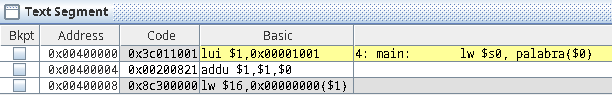
\includegraphics[width=.9\linewidth]{img/c2-5.png}
    \caption{Direcciones de memoria, instrucciones y sus valores en memoria, posteriores al ensamblado del programa dado}
    \label{fig:c2-5}
\end{figure}

Es curioso ver por qué el simulador tradujo la instrucción original en las 3 vistas en la figura anterior. Particularmente porque la instrucción \mintinline{mips}{lw} \textbf{no} es una pseudoinstrucción, sin mencionar que la última de las mencionadas 3 \textit{es una instrucción }\textsl{\mintinline{mips}{lw}}.

Debemos de recordar que la etiqueta \texttt{palabra} apunta a una dirección de memoria, por lo que tiene una longitud de 32 bits. Ya vimos en la sección anterior que es imposible contener un valor de tamaño tal en una sola instrucción, y es justamente por esto que el simulador recurre a un par de instrucciones adicionales para traducir la instrucción en el programa, a código máquina.

De esta forma, vemos en la primera instrucción traducida, el comienzo de un mecanismo muy similar al visto en la traducción de la pseudoinstrucción \mintinline{mips}{li}, donde los 2 bytes más significativos del valor inmediato son cargados en el registro temporal \mintinline{mips}{$at} mediante la instrucción \mintinline{mips}{lui}. Sin embargo, en contraste con el proceso visto en la Cuestión anterior, no se hace uso de la instrucción \mintinline{mips}{ori}.

La segunda de las instrucciones traducidas añade el valor del registro ingresado \mintinline{mips}{$0} (que ya sabemos siempre contendrá un cero) a los dos bytes más altos de \texttt{palabra} cargados en \mintinline{mips}{$at}, pareciendo ignorar los dos bytes menos significativos de \texttt{palabra}. Así luego, la tercera instrucción traducida utiliza como destino al registro así indicado en la instrucción original (\mintinline{mips}{$s0}), y el registro \mintinline{mips}{$at} junto con un valor inmediato \texttt{0x00000000} como dirección de memoria desde la cual cargar, permitiendo usar directamente el valor en \mintinline{mips}{$at} sin modificarlo.

A pesar de la omisión mencionada, como la dirección de \texttt{palabra} en este caso tiene sus dos bytes menos significativos en 0, el código ensamblado funciona correctamente. Por este motivo, podemos probar agregar en el código la declaración de una palabra adicional antes de \texttt{palabra}, que obligue a esta última a ubicarse en una posición de memoria donde sus dos bytes menos significativos sean distintos de cero:

\vspace{7pt}
\inputminted[linenos]{mips}{src/cuestiones/c2-6.asm}
\vspace{7pt}

Tras ensamblar el código con esta modificación, si bien no vemos instrucciones adicionales que consideren los dos bytes que creíamos eran omitidos, resulta que éstos son contemplados a partir del valor inmediato de la tercera instrucción traducida \mintinline{mips}{lw}. Como ésta admite una media palabra como valor inmediato, puede contener aquellos bytes menos significativos y sumárselos a los otros dos más significativos cargados en \mintinline{mips}{$at}, efectivamente representando la dirección de memoria de \texttt{palabra}, cuyo valor quiere cargarse en el registro \mintinline{mips}{$s0}.

Es por esto que vemos en el panel del segmento de texto, que el valor inmediato de \mintinline{mips}{lw} es \texttt{0x00000004}, para contar por el desfase de bytes que tuvo la etiqueta \texttt{palabra} tras agregar la declaración de una variable con la directiva \mintinline{mips}{.word} al comienzo del segmento de datos (\mintinline{mips}{.data}) [Fig. \ref{fig:c2-6}].

\begin{figure}[H]
    \centering
    \captionsetup{justification = centering}
    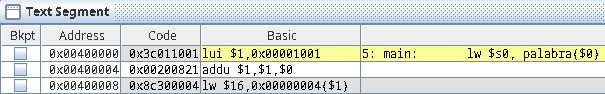
\includegraphics[width=.9\linewidth]{img/c2-6.png}
    \caption{Panel del segmento de texto tras introducir la declaración de una nueva variable del largo de una palabra, anterior a la declaración de \texttt{palabra}}
    \label{fig:c2-6}
\end{figure}

\subsection*{2.7}

\begin{itemize}
    \usemintedstyle{murphy}
    \item \mintinline{mips}{lui $1, 0x00001001} $\rightarrow$ \texttt{0x3c011001} = \texttt{\textcolor{murphy-green-pyg}{001111}00 000\textcolor{murphy-periwinkle-pyg}{00001} \textcolor{murphy-deepsea-pyg}{00010000 00000001}}
    \begin{itemize}
        \item \mintinline{mips}{lui} es la instrucción, su opcode es \texttt{0xF}, abarca los primeros 6 bits.
        \item \mintinline{mips}{$1} es el registro de destino, abarca 5 bits.
        \item \mintinline{mips}{0x00001001} o acortado \mintinline{mips}{0x1001} es un valor inmediato con una longitud de media palabra (últimos 16 bits).
    \end{itemize}

    La instrucción carga en los 16 bits más significativos del registro identificado como \mintinline{mips}{$1}, el valor inmediato \mintinline{mips}{0x1001}.

    \usemintedstyle{default}
    \item \texttt{\textcolor{murphy-green-pyg}{addu} \textcolor{cyan}{\$1}, \textcolor{magenta}{\$1}, \textcolor{Fuchsia}{\$0}} $\rightarrow$ \texttt{0x00200821} = \texttt{\textcolor{murphy-green-pyg}{000000}\textcolor{magenta}{00 001}\textcolor{Fuchsia}{00000} \textcolor{cyan}{00001}000 00\hl{100001}}
    \begin{itemize}
        \item \texttt{\textcolor{murphy-green-pyg}{addu}} es la instrucción, abarca los primeros 6 bits y comparte un opcode \texttt{0x0} con otras instrucciones.
        
        Se identifica de otras instrucciones con dicho opcode a partir de los bits en el campo conocido como \textit{funct}, que en este caso es \texttt{0x21}, y está arriba \hl{resaltado en amarillo}.

        \item \texttt{\textcolor{cyan}{\$1}} es el registro de destino, abarca 5 bits.
        \item \texttt{\textcolor{magenta}{\$1}} y \texttt{\textcolor{Fuchsia}{\$0}} son ambos registros de origen y operandos de la instrucción, abarcan 5 bits cada uno.
    \end{itemize}

    La instrucción escribe en el registro de destino \textcolor{cyan}{\texttt{\$1}}, el resultado de la suma \textit{no signada} (es decir, sin importar el signo) de los números almacenados en los registros de origen \texttt{\textcolor{magenta}{\$1}} y \texttt{\textcolor{Fuchsia}{\$0}}. Sabiendo que \texttt{\textcolor{Fuchsia}{\$0}} siempre contiene el número cero, y que el otro de los registros de origen es el mismo que el registro de destino, entonces el valor no cambia.

\item \texttt{\textcolor{murphy-green-pyg}{lw} \textcolor{cyan}{\$16}, \textcolor{magenta}{0x00000000}(\textcolor{Fuchsia}{\$1})} $\rightarrow$ \texttt{0x8c300000} = \texttt{\textcolor{murphy-green-pyg}{100011}\textcolor{Fuchsia}{00 001}\textcolor{cyan}{10000} \textcolor{magenta}{00000000 00000000}}
    \begin{itemize}
        \item \texttt{\textcolor{murphy-green-pyg}{lw}} es la instrucción, su opcode es \texttt{0x23}, abarca los primeros 6 bits.
        \item \texttt{\textcolor{cyan}{\$16}} es el registro de destino, abarca 5 bits.
        \item \texttt{\textcolor{magenta}{0x00000000}} o acortado \texttt{\textcolor{magenta}{0x0000}} es un valor inmediato con una longitud de media palabra (últimos 16 bits).
        \item \texttt{\textcolor{Fuchsia}{\$1}} es la dirección de un registro cuyo valor debe apuntar a una dirección de memoria (a la que luego se le sumará el valor inmediato en concepto de \textit{offset}). Abarca 5 bits.
    \end{itemize}

    La instrucción carga en el registro de destino \texttt{\textcolor{cyan}{\$16}} (también conocido como \mintinline{mips}{$s0}), el valor contenido en la dirección de memoria obtenida de la suma entre: el valor contenido en el registro \texttt{\textcolor{Fuchsia}{\$1}}, y el valor inmediato proporcionado \texttt{\textcolor{magenta}{0x0000}}.
\end{itemize}

\subsection*{2.8}

Como es de esperarse, al correr el programa, como \texttt{palabra} apunta a la dirección de memoria \texttt{0x10010000}, y el registro \mintinline{mips}{$0} siempre contiene un valor 0; se carga el valor contenido en la dirección \texttt{0x10010000} (o sea, directamente a la que apunta \texttt{palabra}), \texttt{\textbf{0x10203040}}, en el registro de destino \mintinline{mips}{$s0}.

\subsection*{2.9}

Para poder cargar la dirección de un dato en un registro, podemos usar la pseudoinstrucción \mintinline{mips}{la}. De esta forma podemos modificar el programa del ejercicio de manera que haga uso de dicha pseudoinstrucción, pero cumpliendo la misma tarea que el código original:

\vspace{7pt}
\inputminted[linenos]{mips}{src/cuestiones/c2-9.asm}
\vspace{7pt}

Verificando el panel del segmento de texto, podemos ver que la pseudoinstrucción utilizada, de forma prácticamente idéntica a la instrucción \mintinline{mips}{li} vista en las Cuestiones \hyperref[sec:c2-1]{2.1}-\hyperref[sec:c2-4]{2.4}, fue sustituida por las instrucciones \mintinline{mips}{lui} y \mintinline{mips}{ori}. Éstos son utilizados por el programa ensamblado para poder cargar los 2 bytes más significativos, y los 2 menos significativos, en el registro \mintinline{mips}{$t0}, respectivamente.

Como un comentario adicional, mencionar que hacemos uso del registro \mintinline{mips}{$t0} para almacenar la dirección de memoria a la que apunta la etiqueta \texttt{palabra}, ya que los registros comenzados en \textit{t} son generalmente utilizados para almacenar valores temporales. Es por esto la letra con la que comienzan: son \textit{\textbf{t}emporary}.

\subsection*{2.10}

Partiendo del programa ya modificado de la Cuestión anterior, modificarlo nuevamente para cargar en el registro \mintinline{mips}{$s0} la palabra que se encuentra desde \texttt{palabra+1} es tan sencillo como cambiar el valor inmediato de la instrucción \mintinline{mips}{lw}:

\vspace{7pt}
\inputminted[linenos]{mips}{src/cuestiones/c2-10.asm}
\vspace{7pt}

Ahora, en vez de usar el valor \mintinline{mips}{0x0000}, usamos el número \mintinline{mips}{1}, para desfasar la dirección \texttt{+1} posiciones. Así vemos que también podemos usar valores decimales como valor inmediato de la instrucción \mintinline{mips}{lw}.

Dicho esto, al intentar correr el programa, nos encontramos con un error de ejecución en la consola del simulador (Fig. \ref{fig:error-exec-2-10}).

\begin{figure}[H]
    \centering
    \captionsetup{justification = centering}
    \begin{tcolorbox}[fontupper=\small, width=.8\linewidth]
        \begin{Verbatim}[breaklines, breakanywhere, breaksymbol=, breakanywheresymbolpre=, commandchars=\\\{\}]
Error in \textbf{[\textit{redacted}]}/c2-10.asm line 5: Runtime exception at 0x00400008: fetch address not aligned on word boundary 0x10010001

Go: execution terminated with errors.
        \end{Verbatim}
    \end{tcolorbox}
    \caption{Error en la consola del simulador al intentar correr el código modificado}
    \label{fig:error-exec-2-10}
\end{figure}

Resulta que, como venimos insistiendo a lo largo del trabajo, las palabras en la memoria deben estar necesariamente alineadas con direcciones múltiplos de 4. Esto no excluye el acceso a la memoria, por lo que, sabiendo que \texttt{palabra} sí es una dirección de memoria válida, la dirección de memoria \texttt{palabra+1} resulta inválida al no ser múltiplo de 4 (considerando obvio que la dirección de memoria debe ser la del \textbf{primer} byte de la palabra). Debemos de entender que al sumarle un \texttt{1} a la dirección, a partir de cambiar el valor inmediato de la instrucción \mintinline{mips}{lw}, ésto la avanza en una posición, que se corresponde con un byte; no cuatro. 

De hecho, el error nos indica cuál es la dirección de memoria que produjo el error: \textbf{\texttt{0x10010001}}. Si el valor al que apunta \texttt{palabra} es el primero (y único) declarado en el segmento de datos, por defecto su dirección será \texttt{0x10010000}. Fácilmente se puede ver que \texttt{0x10010000} + 1 = \texttt{0x10010001}.

\subsection*{2.11}

Finalmente, para poder guardar los dos bytes de mayor peso (los más significativos) de \texttt{palabra} en \mintinline{mips}{$s0}, podemos ajustar el offset del valor inmediato de la instrucción \mintinline{mips}{lh} en \textit{2} posiciones respecto a la posición de \texttt{palabra}.

Esto funciona ya que al especificar una dirección, como estamos indicando que se cargue una media palabra, la operación será aplicada sobre el byte en la posición utilizada como argumento y la siguiente a ella; son 2 bytes. Por lo tanto, considerando lo explorado en la Cuestión \hyperref[sec:c1-10]{1.10}, sabiendo que MIPS (o al menos el simulador utilizado) almacena los valores bajo el formato \textit{Little-Endian}, implicaría que si utilizamos \texttt{palabra+2} como parámetro a \mintinline{mips}{lh}, los dos bits más significativos de la palabra serían cargados en el registro.

Recordar que \textit{Little-Endian} es un formato/orden donde los bits menos significativos se ubican en las posiciones de memoria más bajas. En este sentido, si no desfásaramos la posición de memoria de \texttt{palabra}, se tomarían los dos bits \textit{menos} significativos. Pues si la palabra comienza en la posición apuntada por la etiqueta, como ésta es la posición de memoria más baja entre las 4 que abarca, bajo el concepto de Little-Endian, resultaría que las primeras dos posiciones se corresponden con los bits de menor peso.

El código resultante es el siguiente:

\vspace{7pt}
\inputminted[linenos]{mips}{src/cuestiones/c2-11.asm}
\vspace{7pt}

Llama la atención que al tratarse de medias palabras, no hay fallos del simulador en cuanto a que la dirección especificada no sea múltiplo de 4. Al parecer, con \textit{halfwords}, las direcciones deben estar alineadas con múltiplos de 2, ya que si intentamos reemplazar la instrucción [\mintinline[escapeinside=||]{mips}{lh $s0, |\hl{2}|($t0)}] con \mintinline[escapeinside=||]{mips}{lh $s0, |\hl{3}|($t0)}, el simulador falla al ejecutar el programa de una forma muy similar a la vista en la Figura \ref{fig:error-exec-2-10}. La única diferencia es que el mensaje advierte sobre el \texttt{halfword boundary} en vez del \texttt{word boundary}.


\begin{center}
\large\textbf{-- \textsl{Carga de bytes (bytes de memoria a registro)} --}
\end{center}

\chapter{Problemas}


\begin{center}
    \Large\textbf{-- Apartado 1 --}
\end{center}

\section{}

\usemintedstyle{autumn}
\inputminted{mips}{src/problemas/1.asm}
\usemintedstyle{default}

En \textcolor{autumn-red-pyg}{\textbf{rojo}} se indican las etiquetas, en \textcolor{autumn-blue-pyg}{\textbf{azul}} las directivas, en \textcolor{autumn-gray-pyg}{\textbf{gris}} los comentarios, y en \textcolor{autumn-teal-pyg}{\textbf{celeste}} las instrucciones.

\section{}

\inputminted{mips}{src/problemas/2.asm}

Utilizo dos directivas \mintinline{mips}{.space} pasándoles el número \textit{80} como argumento pues si una palabra son 4 bytes, y cada vector tiene que tener 20 palabras: $20 \cdot 4\;\text{bytes} = 80\;\text{bytes}$.

\section{}

\inputminted{mips}{src/problemas/3.asm}


\section{}

\inputminted{mips}{src/problemas/4.asm}


\section{}

\inputminted[breaklines, breakbytokenanywhere]{mips}{src/problemas/5.asm}


\section{}

\inputminted{mips}{src/problemas/6.asm}

En ambos casos uso vectors de bytes, ya que los números de la matriz son lo suficientemente pequeños para ser almacenados de esta manera.

Al guardar la matriz por filas, termina resultando en un orden creciente, ya que entendemos que al ``almacenar por filas''. vamos guardando las filas de arriba hacia abajo, y los valores de cada una se almacenarán de forma consecutiva, como se leen de izquierda a derecha.

Mientras, al guardar la matriz por columnas, entendemos que almacenamos las columnas de izquierda a derecha, y que los valores de cada una de ellas se almacenarán de forma consecutiva, como se leen de arriba a abajo.

\begin{figure}[h]
    \centering
    \captionsetup{justification = centering}
    \subfloat[Almacenar por filas]{
        \begin{tabular}{!{\vrule width 1.5pt}c|c|c!{\vrule width 1.5pt}}
            \noalign{\hrule height 1.5pt}
            \rowcolor{LimeGreen!50}
            1 & 2 & 3 \\
            \noalign{\hrule height 1.5pt}
            \rowcolor{Violet!50}
            4 & 5 & 6 \\
            \noalign{\hrule height 1.5pt}
            \rowcolor{RoyalBlue!50}
            7 & 8 & 9 \\
            \noalign{\hrule height 1.5pt}
        \end{tabular}

        $\rightarrow$

        \begin{tabular}{!{\vrule width 1.5pt}>{\columncolor{LimeGreen!50}}c|>{\columncolor{LimeGreen!50}}c|>{\columncolor{LimeGreen!50}}c!{\vrule width 1.5pt}>{\columncolor{Violet!50}}c|>{\columncolor{Violet!50}}c|>{\columncolor{Violet!50}}c!{\vrule width 1.5pt}>{\columncolor{RoyalBlue!50}}c|>{\columncolor{RoyalBlue!50}}c|>{\columncolor{RoyalBlue!50}}c!{\vrule width 1.5pt}}
            \noalign{\hrule height 1.5pt}
            1 & 2 & 3 & 4 & 5 & 6 & 7 & 8 & 9 \\
            \noalign{\hrule height 1.5pt}
        \end{tabular}
    }


    \subfloat[Almacenar por columnas]{
        \begin{tabular}{!{\vrule width 1.5pt}>{\columncolor{LimeGreen!50}}c!{\vrule width 1.5pt}>{\columncolor{Violet!50}}c!{\vrule width 1.5pt}>{\columncolor{RoyalBlue!50}}c!{\vrule width 1.5pt}}
            \noalign{\hrule height 1.5pt}
            1 & 2 & 3 \\
            \hline
            4 & 5 & 6 \\
            \hline
            7 & 8 & 9 \\
            \noalign{\hrule height 1.5pt}
        \end{tabular}

        $\rightarrow$

        \begin{tabular}{!{\vrule width 1.5pt}>{\columncolor{LimeGreen!50}}c|>{\columncolor{LimeGreen!50}}c|>{\columncolor{LimeGreen!50}}c!{\vrule width 1.5pt}>{\columncolor{Violet!50}}c|>{\columncolor{Violet!50}}c|>{\columncolor{Violet!50}}c!{\vrule width 1.5pt}>{\columncolor{RoyalBlue!50}}c|>{\columncolor{RoyalBlue!50}}c|>{\columncolor{RoyalBlue!50}}c!{\vrule width 1.5pt}}
            \noalign{\hrule height 1.5pt}
            1 & 4 & 7 & 2 & 5 & 8 & 3 & 6 & 9 \\
            \noalign{\hrule height 1.5pt}
        \end{tabular}
    }
    \caption{Visualización de las dos formas de almacenar la matriz $A$ del ejercicio}
\end{figure}

\end{document}
